\section{Problem 4}
\textit{Alfa equal 55 degrees is claimed to be a good references – why? B) and why then measure in both 0, 90, 45 and -45 degrees and not 55 degrees?}

To make an evaluation of the environment it is needed to minimize the effect produced by the different polarizations in the received waves in such area. To reduce this effect it can be proved that for a half-length dipole, the mean effective gain (MEG) is the same independently of the cross polarization ratio $XPR$, when said dipole is inclined 55 degrees in its elevation angle.

When said dipole is inclined, it defines a plane (called antenna inclination plane in the bibliography). Subsequently, to evaluate the environment in which the antenna is located, this antenna inclination plane is then rotated in $\Phi$ (the azimuth angle) and the power measurements are performed.

In figure \figref{fig:dipole_inclination} it can be seen the angle $\alpha$ (which is set to 55 degrees in the experiment) and the angle $\Phi$ in which the antenna inclination angle is rotated. It can be mention that in the figure, the vector $L$ is in the antenna inclination plane.


\begin{figure}[!h]
  \centering
  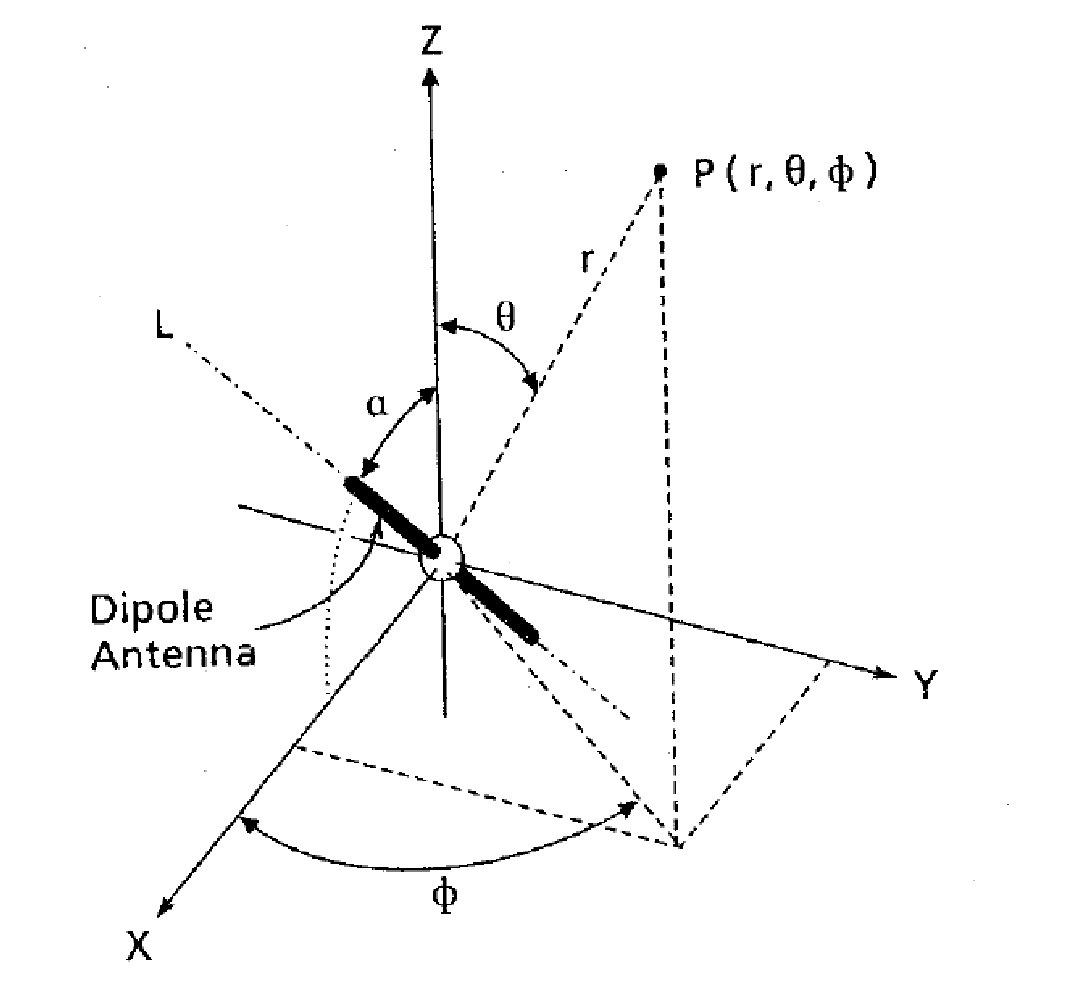
\includegraphics[width=10cm]{dipole_inclination.eps}
  \caption{Figure showing the angles involved in the dipole inclination and rotation (WRITE SOURCE)}
  \label{fig:dipole_inclination}
\end{figure}

The figures \ref{fig:street_nr}and \ref{fig:street_r} represent the situation in which the orientation of the antenna is rotated approximately 90 degrees. The important fact that relies on the different results of the MEG in both cases is the characteristic pattern of the power received in a street. The red ellipses in the figures represents the direction in which the power received is supposed to be higher, resulting in what can be called a 'cannon effect'. Given this, the orientation of the antenna is not negligible in the results and vary with the orientation.


\begin{figure}[!h]
  \centering
  \includegraphics[width=8cm]{street_nr.eps}
  \caption{Figure of the antenna with orientation to $\varphi=0$}
  \label{fig:street_nr}
\end{figure}

\begin{figure}[!h]
  \centering
  \includegraphics[width=8cm]{street_r.eps}
  \caption{Figure of the antenna with different orientation (approximately $\varphi=90$)}
  \label{fig:street_r}
\end{figure}

